\paragraph{}
\textit{Sopra Steria} est une entreprise de services du numérique (ESN) résultant de la fusion, en janvier 2015, de deux des plus anciennes sociétés de services en ingénierie informatique françaises, \textit{Sopra} et \textit{Steria}.

\subsection{1968 - 1985 : Les débuts}

\paragraph{}
Création des sociétés Sopra et Steria respectivement en 1968 et 1969, période marquée par la naissance de l'industrie des services informatiques.

La \textbf{SO}ciété de \textbf{PR}ogrammation et d'\textbf{A}nalyses (Sopra), fondée par Pierre Pasquier et François Odin, est avant tout une entreprise de services de conseils technologiques spécialisée dans l'édition de logiciel. Elle signera, quelques années plus tard, son premier grand contrat d'infogérance bancaire qui marquera son initiation au savoir-faire relatif à la banque. Cela aboutira à la création de la première plateforme bancaire de Sopra qui proposera par la suite des logiciels à destination des banques. Par la suite, l'édition de solutions bancaires deviendra son activité phare avec la mise en production de sa première application concernant les crédits.

La \textbf{S}ocié\textbf{T}é d'\textbf{E}tude et de \textbf{R}éalisation en \textbf{I}nformatique et \textbf{A}utomatisme (Steria) contrôlée par Jean Carteron est aussi une société de services informatiques. L'informatisation de l'Agence France Presse est désignée comme étant l'une des première prouesse de la société qui participera par la suite au développement du minitel en travaillant sur la conception de son architecture.

\subsection{1985 - 2000 : Croissance et entrée en bourse}

\paragraph{}
Sopra repense sa structure industrielle en décidant de se recentrer sur des activités précises telles que l'intégration de systèmes et l'édition de logiciels et décroche son premier grand projet national avec le ministère de l'intérieur. Elle est introduite en Bourse en 1990 et multiplie les contrats ainsi que les acquisitions avec, par exemple, le rachat de \textit{SG2 ingénierie} marquant une forte croissance. Elle profitera de ses performances pour étendre son expertise à l'échelle internationale en s'implentant dans différents pays tels que le Royaume-Uni ou encore l'Allemagne.\\

De même, Steria étend son influence en dehors de la France, jusqu'en Arabie Saoudite où elle réalisera le système informatique de la banque centrale saoudienne. Elle intégrera le marché des transports à son domaine d'expertise, notamment grâce au projet d'automatisation du RER A en France, à Paris. Ses futures acquisitions lui permettront une entrée en Bourse en 1999.\\

\subsection{2000 - 2014 : Transformation numérique}

\paragraph{}
L'essor des technologies du numériques, à savoir l'informatique et internet, provoque une mutation des marchés qui a pour conséquence d'apporter de nombreux clients potentiels à la recherche de partenaires pouvant les accompagner dans leur transformation numérique. Les deux sociétés répondront à cette problématique et développeront leurs activités de conseil. Sopra crééra sa filiale \textit{Axway} regroupant ses activités dans le domaine du progiciel et qui entrera aussi en Bourse de manière autonome en 2011. Toujours fortement impliquée dans le domaine bancaire, elle décidera de créer sa filiale \textit{Sopra Banking Software} en 2012 et réalisera de nombreux projets avec les grands noms du secteur bancaire français (Crédit agricole, Société général, BNP, etc...)\\

Steria, de son côté, se retrouvera dans un contexte économique difficile et vera le prix de son action chuter. Elle continuera malgré tout de multiplier les acquisitions (\textit{Bull} en Europe, \textit{Mummert Consulting} en Allemagne ou encore \textit{Xansa} au Royaume-Uni). Elle remportera plusieurs des plus gros contrats (notamment SSCL pour la gestion du back office de plusieurs ministères de l'administration britannique) de son histoire avec le gouvernement britannique.

\subsection{2014 - 2016 : Fusion absorption}

\paragraph{}

En 2014, Sopra, forte d'une grande croissance, prend la décision d'absorber Steria en devenant actionnaire majoritaire à plus de 90\%. Il s'agit là d'une excellente opportunité misant sur la complémentarité des deux géants de l'informatique aussi bien sur le plan métier que sur le plan géographique. En effet, comme nous l'avons dit plus haut, Steria est très présente au Royaume-Uni contrairement à Sopra. De plus, Sopra se vera ainsi faire l'acquisition de nombreux centres de compétences qui viendront renforcer son écrasante influence à travers l'europe. Les deux entreprises partagent beaucoup de points communs tels que la taille, les domaines d'activités ou encore les objectifs, ce qui constitue un atout majeur concernant leur fusion et leur projets d'avenir. La fusion des deux groupes donne donc naissance à Sopra Steria, une entreprise possédant un poids écrasant, un capital titanesque permettant de gagner la confiance de nombreux clients ainsi qu'une très grande expertise lui permettant de mener à bien beaucoup de projets emblématiques tels que : \\

\begin{figure}[h]
	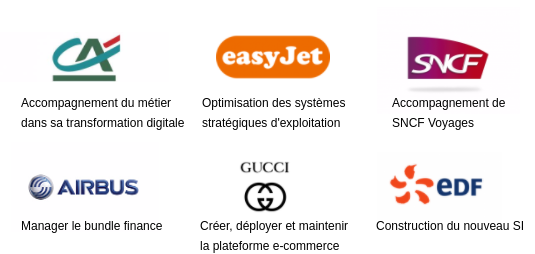
\includegraphics[scale=0.8]{images/entreprise/projetsEmblematiques.png}
	\centering
	\caption{Projets emblématiques}
	\label{projetsEmblematiques}
\end{figure}
		